\ylDisplay{Veetoru} % Ülesande nimi
{Kristian Kuppart} % Autor
{piirkonnavoor} % Voor
{2015} % Aasta
{G 5} % Ülesande nr.
{5} % Raskustase
{
% Teema: Dünaamika
\ifStatement
\begin{wrapfigure}{r}{0.18\textwidth}
 \vspace{-30pt}
 \begin{center}
 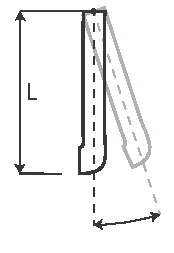
\includegraphics[width=0.18\textwidth]{2015-v2g-05-toru}
 \end{center}
\end{wrapfigure}
Veetoru pikkusega $L$ on kinnitatud seina külge nii, et see saab vertikaaltasandis vabalt pöörelda. Veetoru mass koos seda täitva veega on $M$. Toru ots ristlõikepindalaga $S$ on ülejäänud toruga võrreldes \num{90} kraadi pööratud (vt joonist) ning sellest voolab välja vesi kiirusega $v$ ja tihedusega $\rho$. Kui suure nurga all vertikaali suhtes paikneb toru telg? Raskuskiirenduse väärtus on $g$.
\fi


\ifHint
Toru lõpus järsult pöörav vesi surub toru teatud jõuga külgsuunas. Antud jõud on leitav, kui vaadelda ajaühikus väljuva veehulga impulsimuutu siseneva veega võrreldes.
\fi


\ifSolution
Kui toru otsast voolab välja vesi kiirusega $v$, siis ajaühikus torust väljunud vee hulk on $\frac{\Delta m}{\Delta t}=\rho S v$. Paneme kirja Newtoni II seaduse torust väljunud veehulga jaoks: 
\[ F=\frac{\Delta p}{\Delta t}=\frac{\Delta(mv)}{\Delta t}=v \frac{\Delta m}{\Delta t}. \]
Kuna vesi saab ajaühikus sellise impulsi, peab järelikult Newtoni III seaduse tõttu mõjuma torule sama suur ja vastassuunaline jõud. Paneme kirja jõumomentide tasakaalu võrrandi toru kinnituskoha suhtes: 
\[ \frac{MgL\sin \alpha}{2}=FL. \]
Asendades sisse $\frac{\Delta m}{\Delta t}$ ning avaldades $\alpha$, saame
\[ \alpha=\arcsin \left(\frac{2\rho v^2 S}{Mg}\right). \]
\fi


\ifEngStatement
% Problem name: Water pipe
\begin{wrapfigure}[7]{r}{0.15\textwidth}
  \vspace{-35pt}
  \begin{center}
    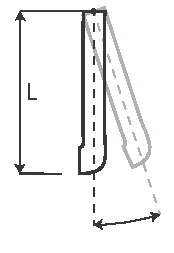
\includegraphics[width=0.18\textwidth]{2015-v2g-05-toru}
  \end{center}
  \vspace*{-10pt}
\end{wrapfigure}
A water pipe with a length $L$ is fixed to a wall so that it can freely rotate on the vertical plane. The water pipe’s mass together with the water it is filled with is $M$. The cross-sectional area of the pipe’s end is $S$. The end is turned 90 degrees with respect to the rest of the pipe (see figure). Water flows out of the end of the pipe with a speed $v$ and density $\rho$. What is the angle between the vertical direction and the pipe’s axis? Gravitational acceleration is $g$.
\fi


\ifEngHint
The sharply turning water at the end of the pipe presses the pipe sideways with a certain force. This force can be found when you observe the momentum change of the exiting water per unit of time compared to the entering water.
\fi


\ifEngSolution
If water with a speed $v$ flows out of the pipe’s end then the amount of water that exits the pipe per unit of time is $\frac{\Delta m}{\Delta t}=\rho S v$. We write down the Newton’s second law for the amount of water exiting the pipe:
\[ F=\frac{\Delta p}{\Delta t}=\frac{\Delta(mv)}{\Delta t}=v \frac{\Delta m}{\Delta t}. \] 
Because the water obtains such a momentum per unit of time then according to the Newton’s third law an equal force with the opposite direction should be applied to the pipe. We write down the equation for torque balance with respect to the pipe’s attachment point:
\[ \frac{MgL\sin \alpha}{2}=FL. \] 
Replacing $\frac{\Delta m}{\Delta t}$ into the equation and expressing $\alpha$ we get
\[ \alpha=\arcsin (\frac{2\rho v^2 S}{Mg}). \]
\fi
}